\index{reference cells}

The following five reference cells are covered by the UFC specification:
the reference \emph{interval},
the reference \emph{triangle},
the reference \emph{quadrilateral},
the reference \emph{tetrahedron} and
the reference \emph{hexahedron} (see Table~\ref{tab:ufc_reference_cells}).

\begin{table}
\linespread{1.2}\selectfont
  \begin{center}
    \begin{tabular}{|l|c|c|c|}
      \hline
      Reference cell & Dimension & \#Vertices & \#Facets \\
      \hline
      \hline
      The reference interval      & 1 & 2 & 2 \\
      \hline
      The reference triangle      & 2 & 3 & 3 \\
      \hline
      The reference quadrilateral & 2 & 4 & 4 \\
      \hline
      The reference tetrahedron   & 3 & 4 & 4 \\
      \hline
      The reference hexahedron    & 3 & 8 & 6 \\
      \hline
    \end{tabular}
    \caption{Reference cells covered by the UFC specification.}
    \label{tab:ufc_reference_cells}
  \end{center}
\end{table}

The UFC specification assumes that each cell in a finite element mesh
is always isomorphic to one of the reference cells.

\section{The reference interval}
\index{interval}

The reference interval is shown in Figure~\ref{fig:interval} and is
defined by its two vertices with coordinates as specified in
Table~\ref{tab:interval,vertices}.

\begin{figure}
  \begin{center}
    \psfrag{0}{$0$}
    \psfrag{1}{$1$}
    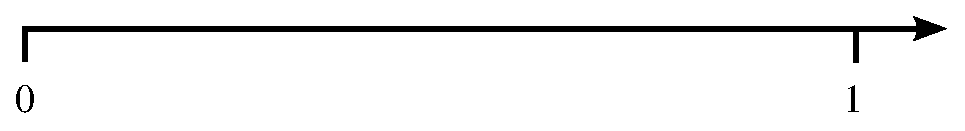
\includegraphics[width=10cm]{eps/interval.eps}
    \caption{The reference interval.}
    \label{fig:interval}
  \end{center}
\end{figure}

\begin{table}
\linespread{1.2}\selectfont
  \begin{center}
    \begin{tabular}{|c|c|}
      \hline
      Vertex & Coordinate \\
      \hline
      \hline
      $v_0$ & $x = 0$ \\
      \hline
      $v_1$ & $x = 1$ \\
      \hline
    \end{tabular}
    \caption{Vertex coordinates of the reference interval.}
    \label{tab:interval,vertices}
  \end{center}
\end{table}

\section{The reference triangle}
\index{triangle}

The reference triangle is shown in Figure~\ref{fig:triangle} and is
defined by its three vertices with coordinates as specified in
Table~\ref{tab:triangle,vertices}.

\begin{figure}
  \begin{center}
    \psfrag{v0}{$(0, 0)$}
    \psfrag{v1}{$(1, 0)$}
    \psfrag{v2}{$(0, 1)$}
    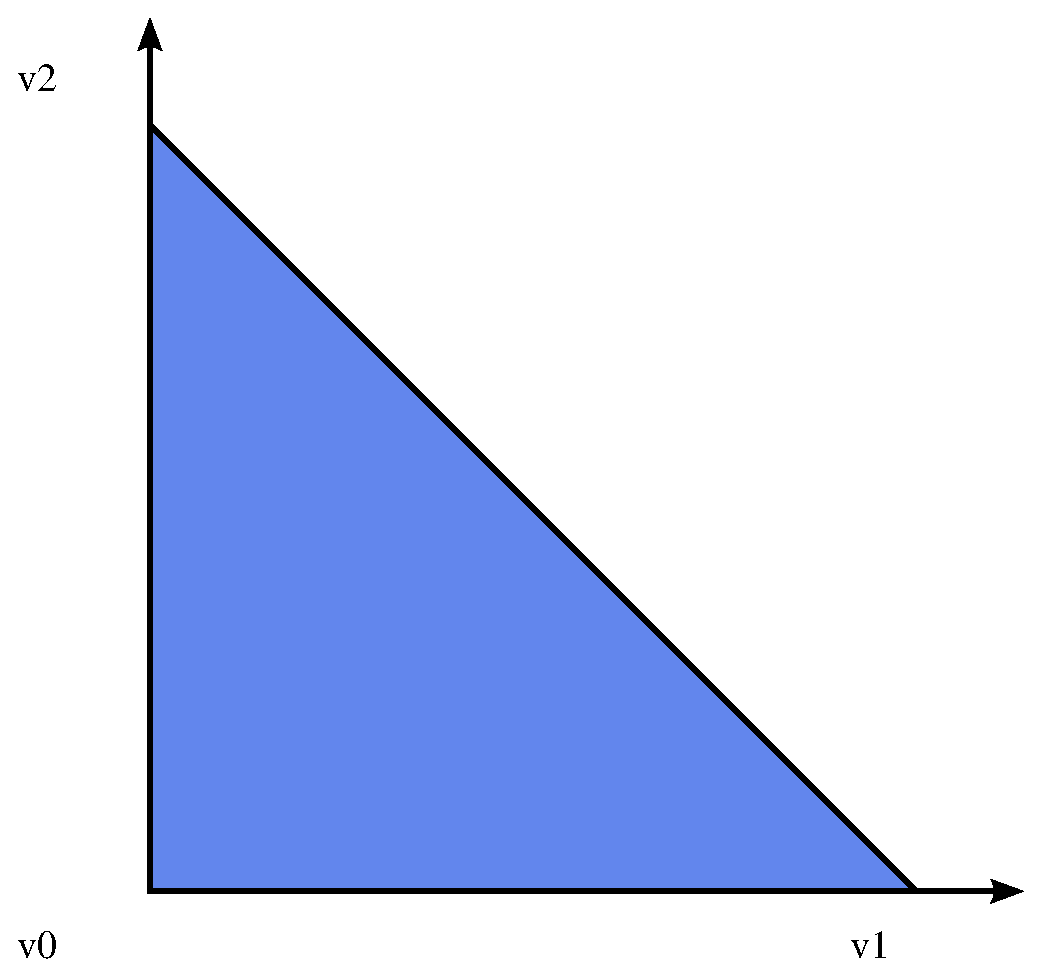
\includegraphics[width=8cm]{eps/triangle.eps}
    \caption{The reference triangle.}
    \label{fig:triangle}
  \end{center}
\end{figure}

\begin{table}
\linespread{1.2}\selectfont
  \begin{center}
    \begin{tabular}{|c|c|}
      \hline
      Vertex & Coordinate \\
      \hline
      \hline
      $v_0$ & $x = (0, 0)$ \\
      \hline
      $v_1$ & $x = (1, 0)$ \\
      \hline
      $v_2$ & $x = (0, 1)$ \\
      \hline
    \end{tabular}
    \caption{Vertex coordinates of the reference triangle.}
    \label{tab:triangle,vertices}
  \end{center}
\end{table}

\section{The reference quadrilateral}
\index{quadrilateral}

The reference quadrilateral is shown in Figure~\ref{fig:quadrilateral}
and is defined by its four vertices with coordinates as specified in
Table~\ref{tab:quadrilateral,vertices}.

\begin{figure}
  \begin{center}
    \psfrag{v0}{$(0, 0)$}
    \psfrag{v1}{$(1, 0)$}
    \psfrag{v2}{$(1, 1)$}
    \psfrag{v3}{$(0, 1)$}
    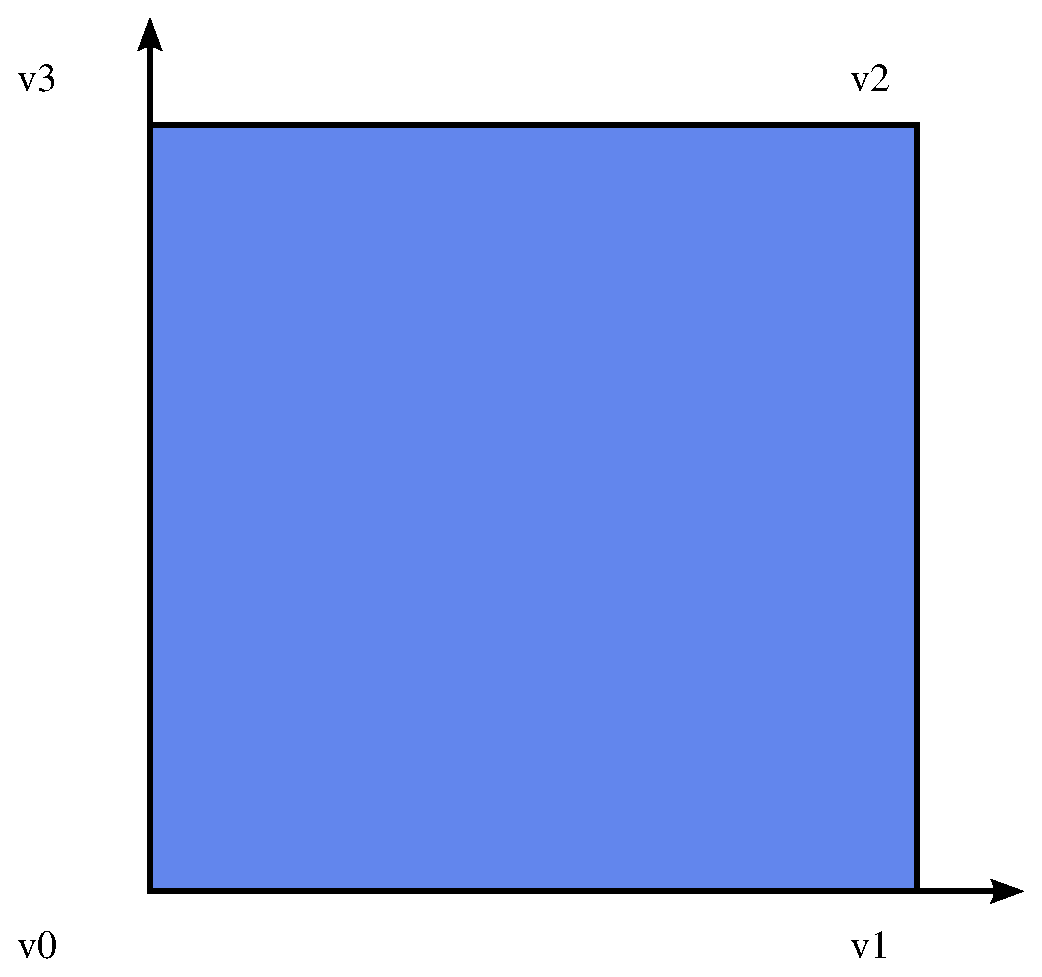
\includegraphics[width=8cm]{eps/quadrilateral.eps}
    \caption{The reference quadrilateral.}
    \label{fig:quadrilateral}
  \end{center}
\end{figure}

\begin{table}
\linespread{1.2}\selectfont
  \begin{center}
    \begin{tabular}{|c|c|}
      \hline
      Vertex & Coordinate \\
      \hline
      \hline
      $v_0$ & $x = (0, 0)$ \\
      \hline
      $v_1$ & $x = (1, 0)$ \\
      \hline
      $v_2$ & $x = (1, 1)$ \\
      \hline
      $v_3$ & $x = (0, 1)$ \\
      \hline
    \end{tabular}
    \caption{Vertex coordinates of the reference quadrilateral.}
    \label{tab:quadrilateral,vertices}
  \end{center}
\end{table}

\section{The reference tetrahedron}
\index{tetrahedron}

The reference tetrahedron is shown in Figure~\ref{fig:tetrahedron} and
is defined by its four vertices with coordinates as specified in
Table~\ref{tab:tetrahedron,vertices}.

\begin{figure}
  \begin{center}
    \psfrag{v0}{$(0, 0, 0)$}
    \psfrag{v1}{$(1, 0, 0)$}
    \psfrag{v2}{$(0, 1, 0)$}
    \psfrag{v3}{$(0, 0, 1)$}
    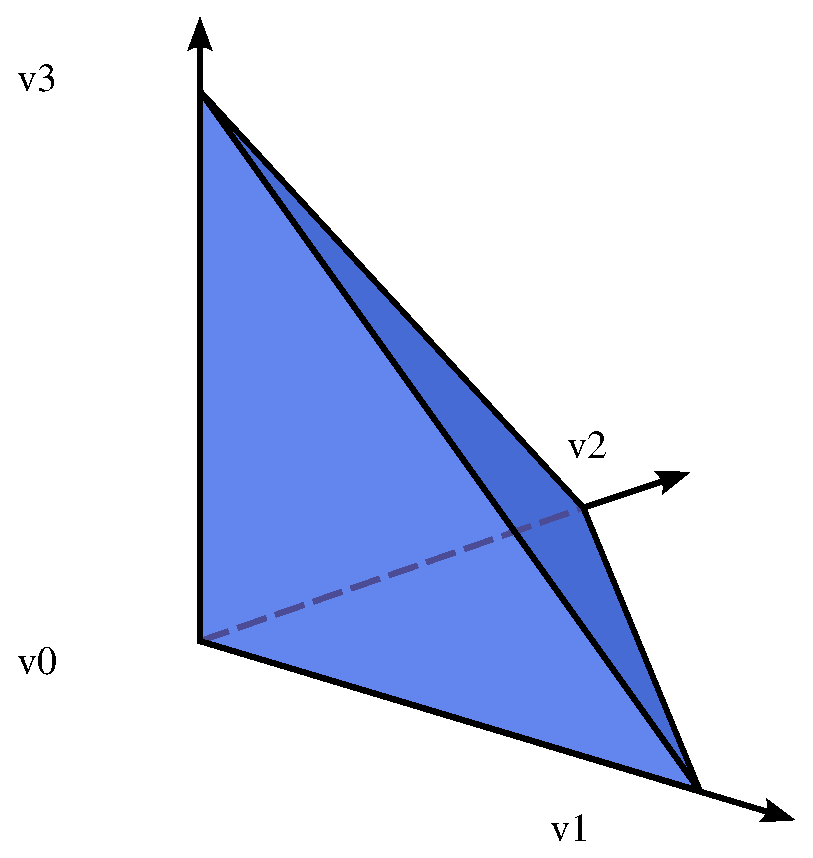
\includegraphics[width=6cm]{eps/tetrahedron.eps}
    \caption{The reference tetrahedron.}
    \label{fig:tetrahedron}
  \end{center}
\end{figure}

\begin{table}
\linespread{1.2}\selectfont
  \begin{center}
    \begin{tabular}{|c|c|}
      \hline
      Vertex & Coordinate \\
      \hline
      \hline
      $v_0$ & $x = (0, 0, 0)$ \\
      \hline
      $v_1$ & $x = (1, 0, 0)$ \\
      \hline
      $v_2$ & $x = (0, 1, 0)$ \\
      \hline
      $v_3$ & $x = (0, 0, 1)$ \\
      \hline
    \end{tabular}
    \caption{Vertex coordinates of the reference tetrahedron.}
    \label{tab:tetrahedron,vertices}
  \end{center}
\end{table}

\section{The reference hexahedron}
\index{hexahedron}

The reference hexahedron is shown in Figure~\ref{fig:hexahedron} and
is defined by its eight vertices with coordinates as specified in
Table~\ref{tab:hexahedron,vertices}.

\begin{figure}
\linespread{1.2}\selectfont
  \begin{center}
    \psfrag{v0}{$(0, 0, 0)$}
    \psfrag{v1}{$(1, 0, 0)$}
    \psfrag{v2}{$(1, 1, 0)$}
    \psfrag{v3}{$(0, 1, 0)$}
    \psfrag{v4}{$(0, 0, 1)$}
    \psfrag{v5}{$(1, 0, 1)$}
    \psfrag{v6}{$(1, 1, 1)$}
    \psfrag{v7}{$(0, 1, 1)$}
    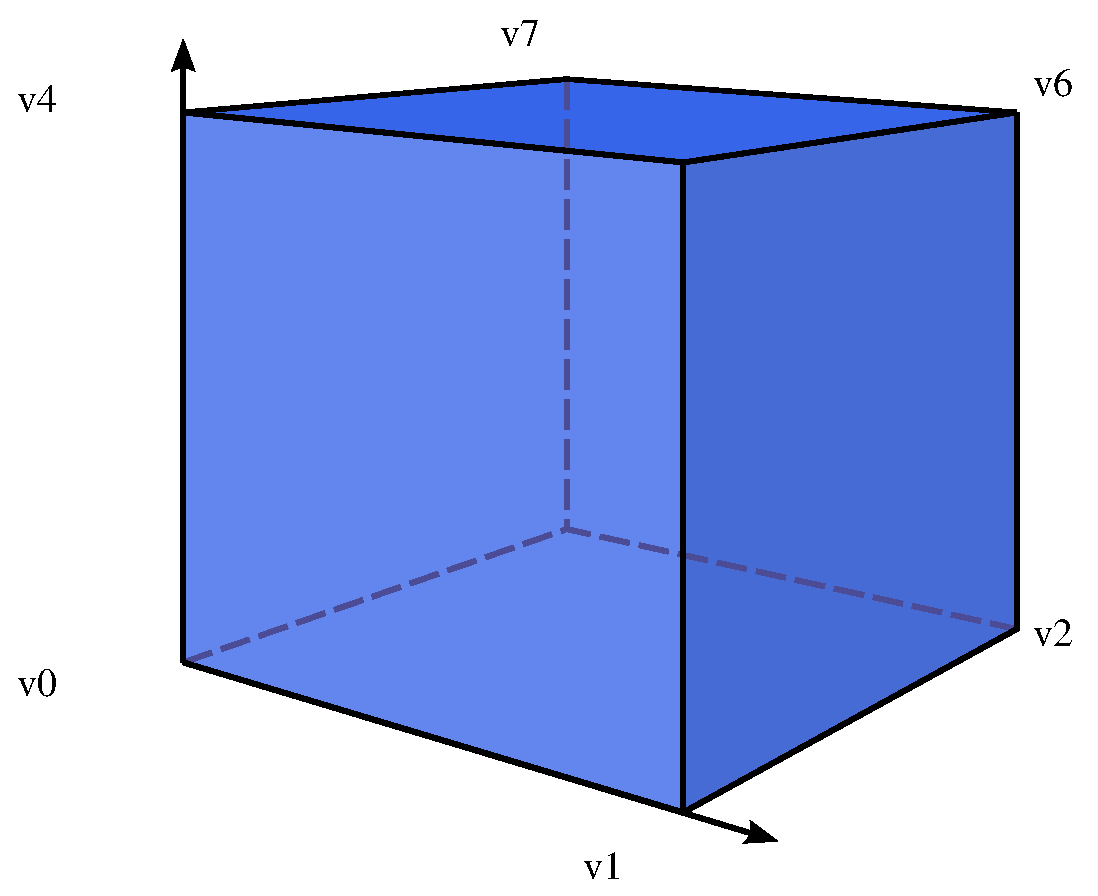
\includegraphics[width=9cm]{eps/hexahedron.eps}
    \caption{The reference hexahedron.}
    \label{fig:hexahedron}
  \end{center}
\end{figure}

\begin{table}
\linespread{1.2}\selectfont
  \begin{center}
    \begin{tabular}{|c|c|}
      \hline
      Vertex & Coordinate \\
      \hline
      \hline
      $v_0$ & $x = (0, 0, 0)$ \\
      \hline
      $v_1$ & $x = (1, 0, 0)$ \\
      \hline
      $v_2$ & $x = (1, 1, 0)$ \\
      \hline
      $v_3$ & $x = (0, 1, 0)$ \\
      \hline
    \end{tabular}
    \begin{tabular}{|c|c|}
      \hline
      Vertex & Coordinate \\
      \hline
      \hline
      $v_4$ & $x = (0, 0, 1)$ \\
      \hline
      $v_5$ & $x = (1, 0, 1)$ \\
      \hline
      $v_6$ & $x = (1, 1, 1)$ \\
      \hline
      $v_7$ & $x = (0, 1, 1)$ \\
      \hline
    \end{tabular}
    \caption{Vertex coordinates of the reference hexahedron.}
    \label{tab:hexahedron,vertices}
  \end{center}
\end{table}
